
\begin{figure}[H]
    \centering
    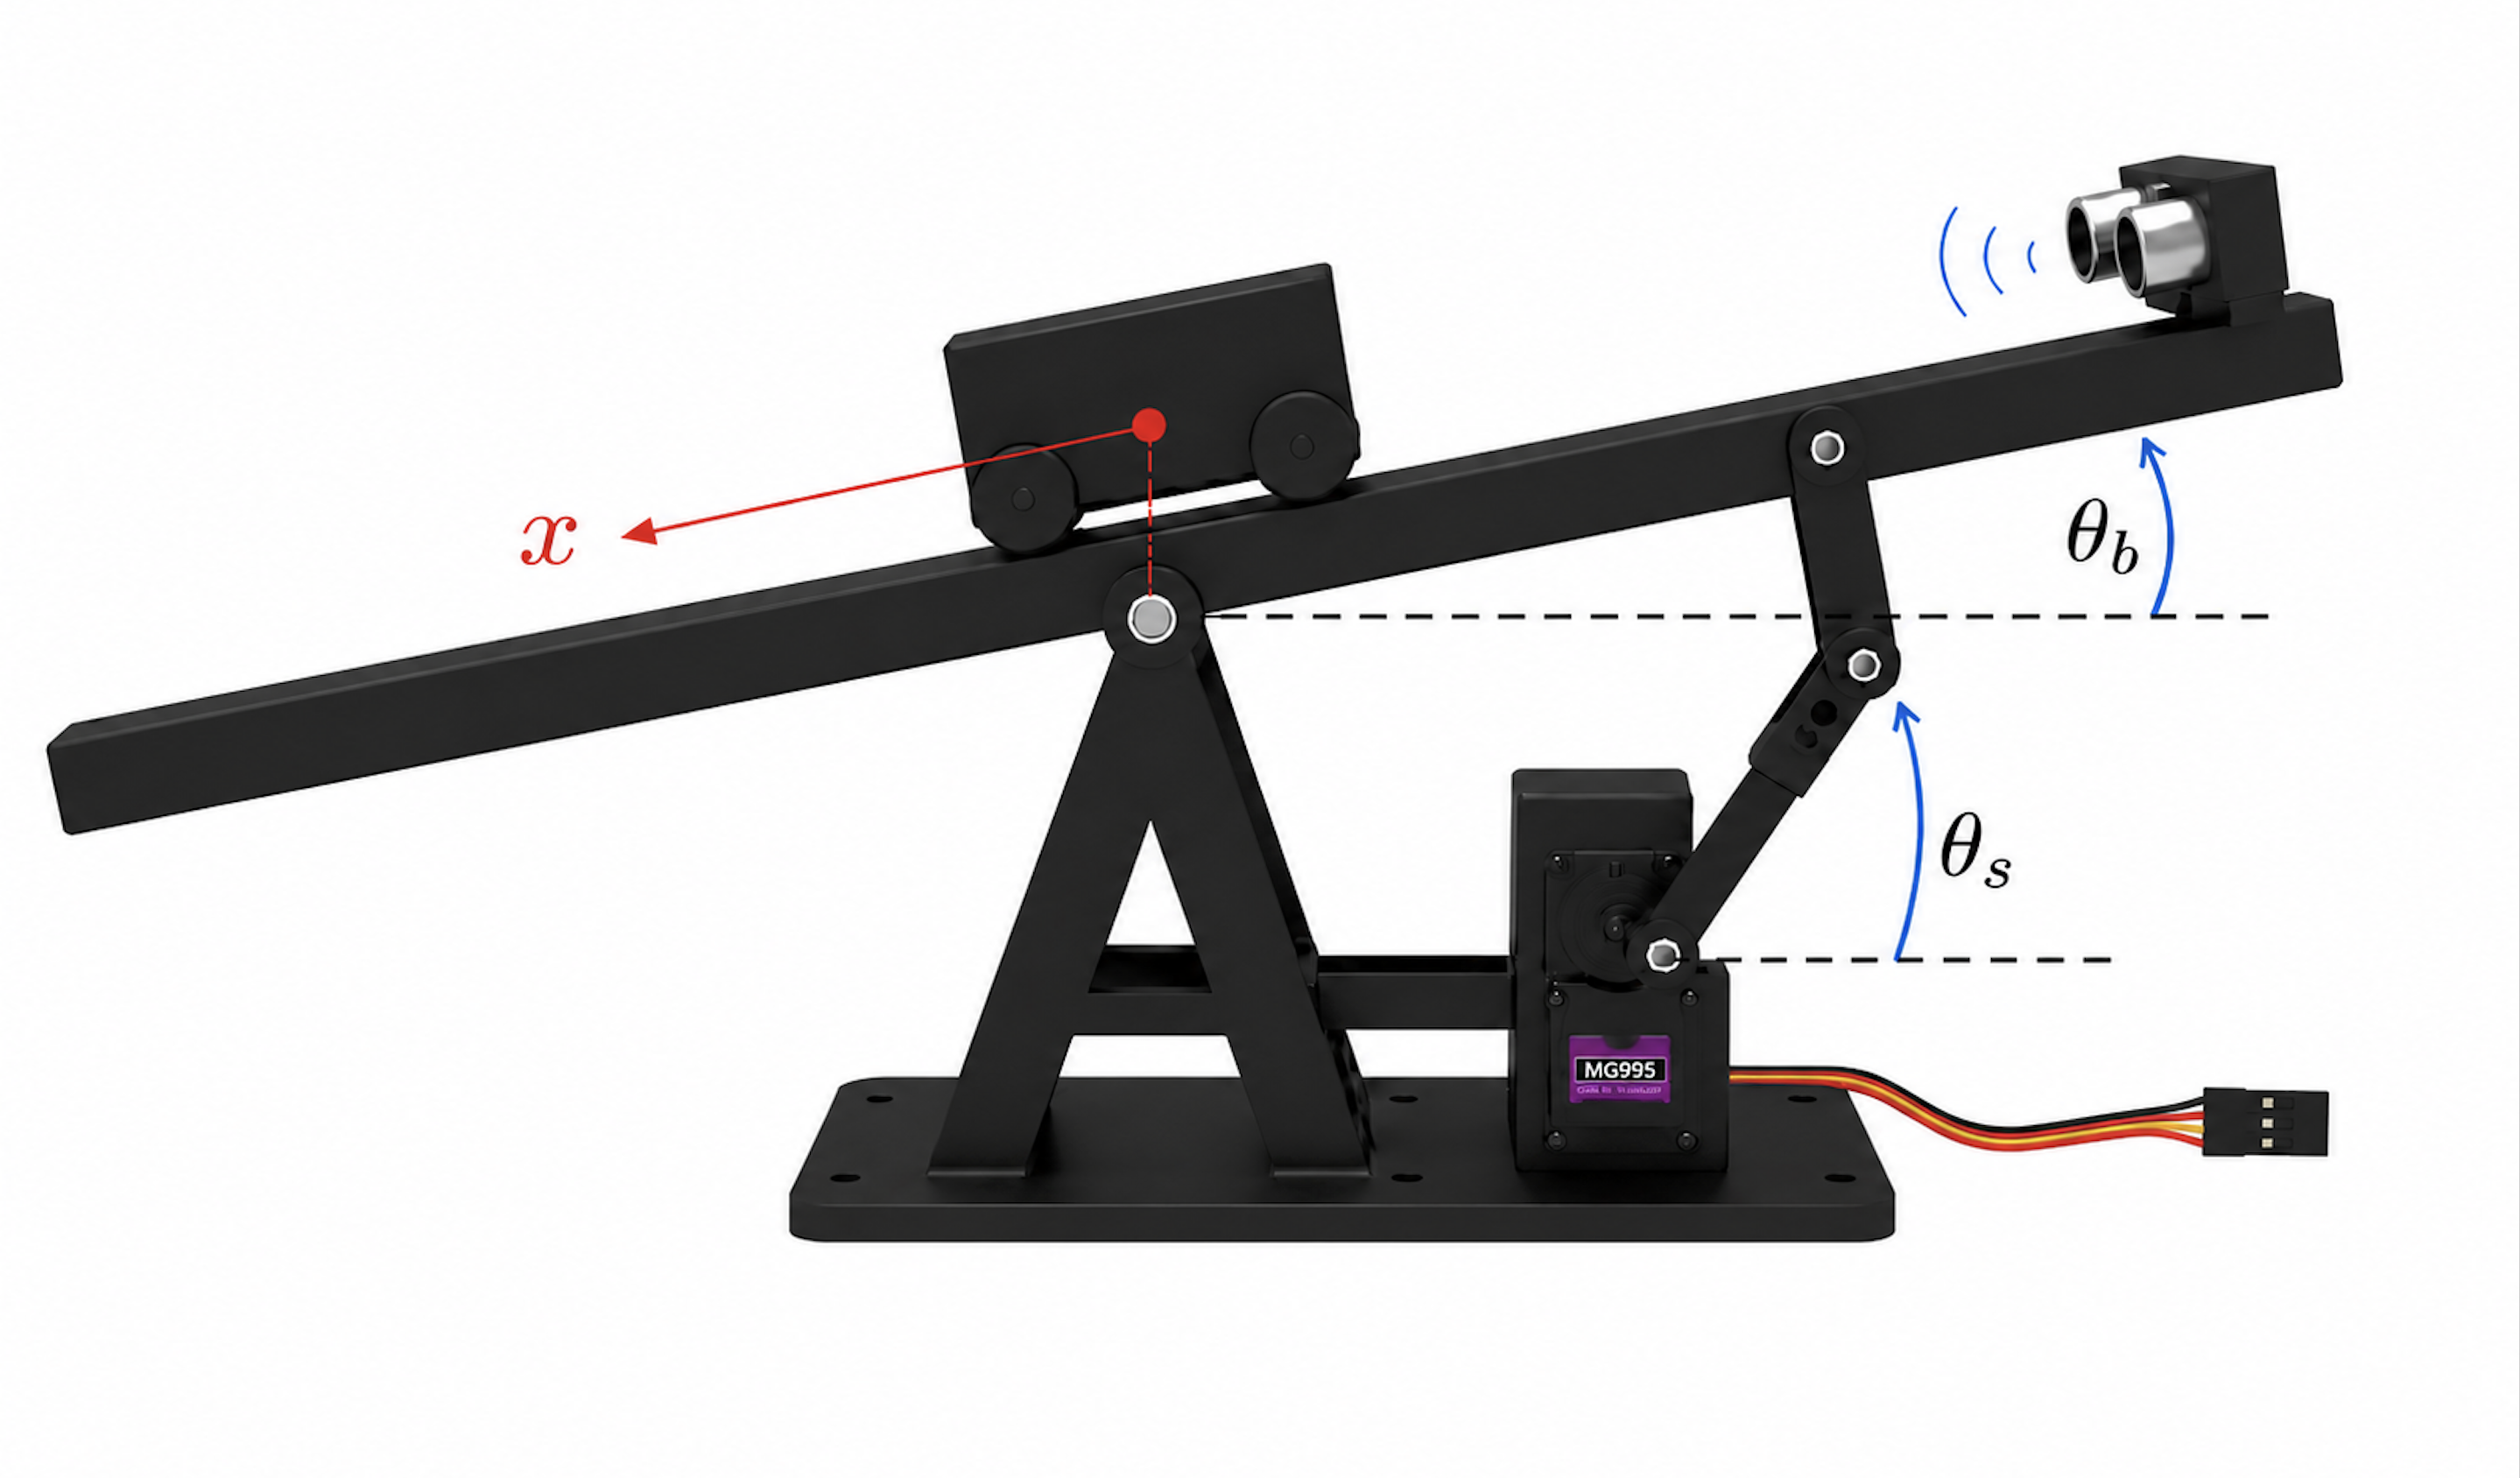
\includegraphics[width=0.8\textwidth]{img/planta.png}
    \caption{Sistema de referencia}
    \label{fig:sistema de referencia}
\end{figure}


Se tiene una barra de \SI{40}{\centi \meter} de longitud controlada por un servomotor sobre la cual se apoya un carrito. Mirando el servomotor de frente se considerna los $x$ positivos hacia la izquierda y los ángulos positivos en sentido antihorario. El origen de coordenadas para la posición es el centro de la barra y el ángulo $\theta_b = 0$ se produce para la barra horizontal. La \autoref{fig:sistema de referencia} ilustra el sistema de referencia adoptado.

Puede definirse un sistema en el que el ángulo comandado al servomotor $u$ es la entrada y la posición del carro es la salida. Se linealizó al mismo en torno al punto de equilibrio $(\theta_b, x) = (0, 0)$ y se halló su representación en espacio de estados.

\begin{minipage}{0.4\textwidth}
    \[
    \begin{cases}
    x_1 = \theta_b : \text{ángulo de la barra} \\
    x_2 = \dot{\theta}_b : \text{velocidad angular de la barra} \\
    x_3 = x : \text{posición del carro} \\
    x_4 = \dot{x} : \text{velocidad del carro}
    \end{cases}
    \]
\end{minipage}%
\begin{minipage}{0.4\textwidth}
\centering
    \begin{equation}
        x =
        \begin{bmatrix}
        x_1 \\
        x_2 \\
        x_3 \\
        x_4
        \end{bmatrix}
        \label{eq:vector de estados}
    \end{equation}
\end{minipage}

La \autoref{eq:vector de estados} muestra el vector de estados adoptado para este problema, en donde las dos primeras variables están asociadas al ángulo de la barra y las dos últimas a la posición del carro. Para este sistema de referencia y este vector de estados ya se había llegado a una representación del sistema en espacio de estados, la cual se repite aquí. 

\[
A=
\begin{bmatrix}
0 & 1 & 0 & 0 \\
-33,1549 & -9,7360 & 0 & 0 \\
0 & 0 & 0 & 1 \\
35,9445 & 0 & 0 & -10
\end{bmatrix}
\qquad
B=
\begin{bmatrix}
0 \\
11,4345 \\
0 \\
0
\end{bmatrix}
\]

\[
C=
\begin{bmatrix}
0 & 0 & 1 & 0
\end{bmatrix}
\qquad
D=
\begin{bmatrix}
0
\end{bmatrix}
\]

Cabe aclarar que este conjunto de matrices es válido si se consider que la salida del sistema es la posición del carro. Si además se quiere considerar el ángulo de la barra como salida, debe reemplazarse la matriz $C$ por: 

\[
C = \begin{bmatrix}
    0 & 0 & 1 & 0 \\
    1 & 0 & 0 & 0 
\end{bmatrix}
\]
.

Por último, de esta representación en espacio de estados puede obtenerse una función de transferencia.

\begin{equation}
\begin{aligned}
P(s) &= \frac{X(s)}{\Theta_s(s)}
      = \frac{k}{s(s-p_1)(s-p_2)(s-p_3)} \\
     &= \frac{410,7144}
{s\left(s+4,8680-3,0753j\right)\left(s+4,8680+3,0753j\right)(s+10)}
\end{aligned}
\end{equation}